\iffalse
\documentclass[journal,10pt,twocolumn]{article}
\usepackage{graphicx}
\usepackage[margin=0.5in]{geometry}
\usepackage[cmex10]{amsmath}
\usepackage{array}
\usepackage{booktabs}
\usepackage{mathtools}
\usepackage{multicol}
\usepackage[utf8]{inputenc}
\title{\textbf{Conic section Assignment}}
\author{Thoutu Rahul Raj}
\date{October 2022}


\providecommand{\norm}[1]{\left\lVert#1\right\rVert}
\providecommand{\abs}[1]{\left\vert#1\right\vert}
\let\vec\mathbf
\newcommand{\myvec}[1]{\ensuremath{\myvec{#1}}}
\newcommand{\mydet}[1]{\ensuremath{\begin{vmatrix}#1\end{vmatrix}}}
\providecommand{\brak}[1]{\ensuremath{\left(#1\right)}}
\providecommand{\lbrak}[1]{\ensuremath{\left(#1\right.}}
\providecommand{\rbrak}[1]{\ensuremath{\left.#1\right)}}
\providecommand{\sbrak}[1]{\ensuremath{{}\left[#1\right]}}

\begin{document}
\maketitle
\section{Problem Statement}
Find the equation of the circle passing through the points (2,3) and (-1,1) and whose centre is on the line $x-3y-11=0$
\fi
\solution See Fig. 
	\begin{figure}[!ht]
		\centering
 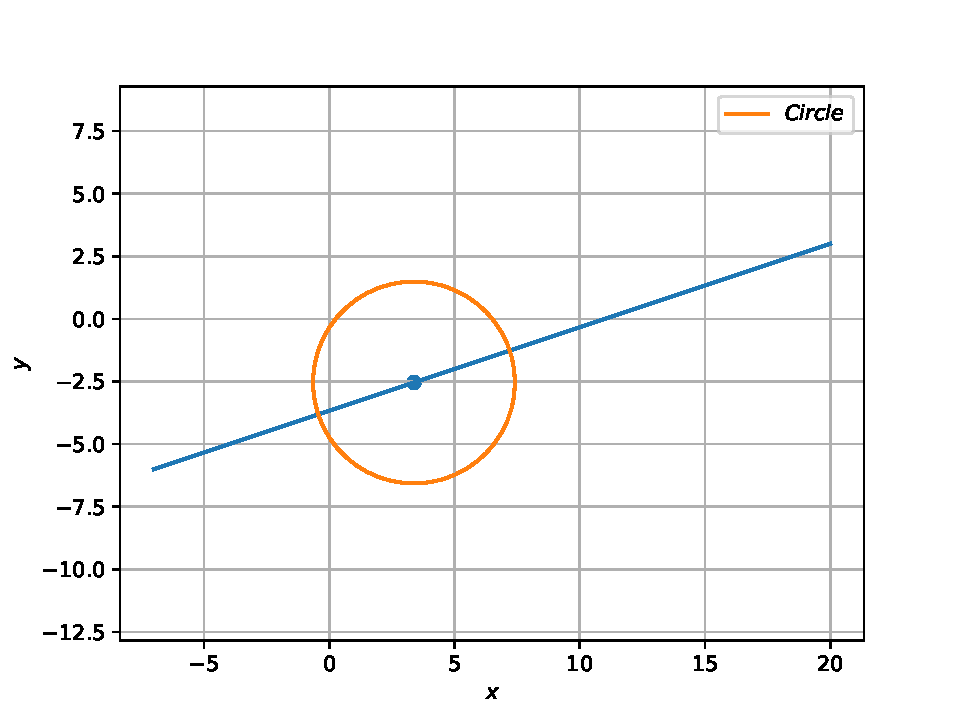
\includegraphics[width=\columnwidth]{chapters/11/11/1/11/figs/fig.pdf}
		\caption{}
		\label{fig:11/11/1/11}
  	\end{figure}
\iffalse
}
\section{Solution}
To Find : The equation of circle.
Given , points passing through circle (2,3) and (-1,1), And equation of line passing through the center of circle x-3y-11=0
\begin{align}
    \vec{x}^{\top}\vec{V}\vec{x}+2\vec{u}^{\top}\vec{x}+f=0\\
	\vec{V} &= \myvec{1 & 0\\0 & 1},
	\\
	\vec{u} &= \myvec{h\\k},
	\\
	f &= f
\end{align}


which is the equation of a circle. 
And h,k,C are unknown values we should find
\fi
From 
	\eqref{eq:circ-eq}, and the given information, 
\begin{align}
	\norm{\vec{P}}^2 + 2 \vec{u}^{\top}\vec{P} + f &= 0
	\\
	\norm{\vec{Q}}^2 + 2 \vec{u}^{\top}\vec{Q} + f &= 0
	\\
	-\vec{n}^{\top}\vec{u} &=c
\end{align}
by noting that the centre of the circle is $-\vec{u}$.
Substituting numerical values, we obtain the matrix equation
\begin{align}
	\label{eq:vertex_system}
	\myvec{4&6&1\\-2& 2&1\\-1& 3&0}\myvec{\vec{u}\\f} = \myvec{-13\\-2 \\11}\\
\end{align}
The augmented matrix for \eqref{eq:vertex_system} can be expressed as
\begin{align}
	\xleftrightarrow[]{1/4 R_1 \leftrightarrow R_1}\myvec{1&3/2&.1/4&\vrule&-13/4\\-2&2&1&\vrule&-2\\-1&3&0&\vrule&11}
\end{align}
which can be reduced to echelon form using row operations to obtain 
\iffalse
\begin{align}
		\xleftrightarrow[]{-1/2R_2 \leftrightarrow R_2}
		\myvec{1&3/2&1/4&\vrule&-13/4\\1&-1&-1/2&\vrule&1\\-1&3&0&\vrule&11}\\
	     \xleftrightarrow[]{-1R_3 \leftrightarrow R_3}	
\myvec{1&3/2&1/4&\vrule&-13/4\\1&-1&-1/2&\vrule&1\\1&-3&0&\vrule&-11}\\
		\xleftrightarrow[]{R_2-1.R_1 \leftrightarrow R_2}
		\myvec{1&3/2&1/4&\vrule&-13/4\\0&-5/2&-3/4&\vrule&17\\1&-3&0&\vrule&-11}\\
	     \xleftrightarrow[]{R_3-1.R_1 \leftrightarrow R_3}
	     \myvec{1&3/2&1/4&\vrule&-13/4\\0&-5/2&-3/4&\vrule&17/4\\0&9/2&-1/4&\vrule&-31/4}\\
	     \xleftrightarrow[]{-2/5R_2 \leftrightarrow R_2}
	  \myvec{1&3/2&1/4&\vrule&-13/4\\0&1&3/10&\vrule&17/10\\0&9/2&-1/4&\vrule&-31/4}
\end{align}
\begin{align}
	      \xleftrightarrow[]{-2/9R_3 \leftrightarrow R_3}	
\myvec{1&3/2&1/4&\vrule&-13/4\\1&-1&-1/2&\vrule&1\\1&-3&0&\vrule&-11}\\
		\xleftrightarrow[]{R_3-1.R_2 \leftrightarrow R_3}
\myvec{1&3/2&1/4&\vrule&-13/4\\0&1&3/10&\vrule&-17/10\\0&0&-11/45&\vrule&154/45}\\		
	     \xleftrightarrow[]{-45/11R_3 \leftrightarrow R_3}
	     \myvec{1&3/2&1/4&\vrule&-13/4\\0&1&3/10&\vrule&-17/10\\0&0&1&\vrule&-14}\\
	     \xleftrightarrow[]{R_2-3/10R_3 \leftrightarrow R_2}
	     \myvec{1&3/2&1/4&\vrule&-13/4\\0&1&0&\vrule&5/2\\0&0&1&\vrule&-14}\\	
	      \xleftrightarrow[]{R_1-1/4R_3 \leftrightarrow R_1}
	      	     \myvec{1&3/2&0&\vrule&1/4\\0&1&0&\vrule&5/2\\0&0&1&\vrule&-14}\\
	       \xleftrightarrow[]{R_1-3/2R_2 \leftrightarrow R_1}	
\myvec{1&0&0&\vrule&-7/2\\0&1&0&\vrule&5/2\\0&0&1&\vrule&-14}\\
\end{align}
yielding 
\fi
\begin{align}
\vec{u}=\myvec{-7/2 \\5/2 },
f=-14
\end{align}
\iffalse
\end{align}
from u and f we can find radius
\begin{align}
 r = \sqrt{\norm{\vec{(u)}}^2-f} 
\end{align}
\begin{align}
r = \sqrt{65/4}
\end{align}
And, from them we can find the equation of circle.\\
 \begin{align}
\vec{x}^{\top}\vec{V}\vec{x}+2\vec{u}^{\top}\vec{x}+f=0
\end{align}	
$\vec{V}$ = $\myvec{
 1 & 0\\
 0 & 1
 }$, 
  $\vec{u}$=$\vec{\myvec{7/2 \\-5/2 }}$
  f = 14
steps for constructing above figure are:  
\begin{center}
\begin{tabular}{|c|c|c|}
	\hline
	\textbf{Symbol}&\textbf{Value}&\textbf{Description}\\
	\hline
	$r$&$\sqrt{65/4}$&Radius of the circle\\
	\hline
	\textbf{C}&$\
	\myvec{
		7/2 \\
		-5/2 \\
	}$
	&center of circle\\
	\hline
\end{tabular}
\end{center}
\vspace{1mm}

\section{ Construction}
%\includegraphics[scale=0.5]{../Documents/co.pdf} 
%\includegraphics[scale=0.5]{co.pdf} 
%\vspace{3mm}
%\url{https://github.com/9705701645/FWC/blob/main/co.py}
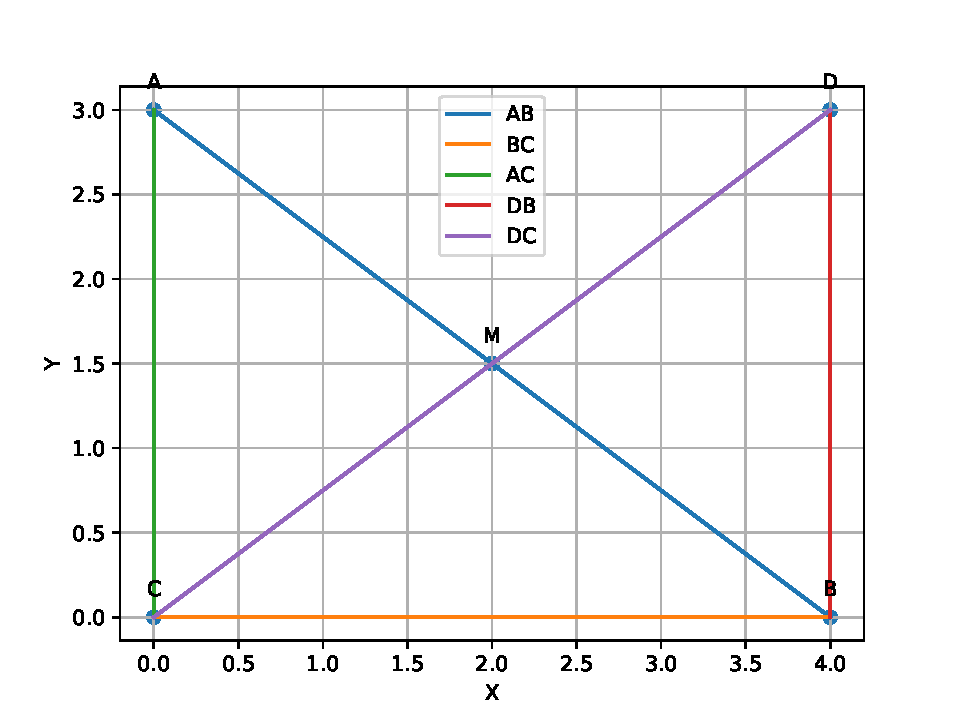
\includegraphics[scale=1]{fig.pdf} 
%\begin{multicols}
 %Download the code \\
%\href{https://github.com/9705701645/FWC/blob/main/co.py}{Assignment-5}.
%\end{multicols}
\end{document}


\fi
